\documentclass[10pt,a4paper]{article}
\usepackage[utf8]{inputenc}
\usepackage[T1]{fontenc}
\usepackage[margin=1.8cm,top=2.6cm,bottom=2.2cm]{geometry}
\usepackage{parskip}
\usepackage{microtype}
\usepackage{amsmath,amssymb,mathtools}
\usepackage{array,booktabs,tabularx}
\usepackage[table]{xcolor}
\usepackage{graphicx,float}
\usepackage{titlesec}
\usepackage{enumitem}
\usepackage{fancyhdr}
\usepackage{tcolorbox}
\usepackage[colorlinks=true,linkcolor=black,citecolor=black,urlcolor=blue!55!black,breaklinks=true]{hyperref}
\urlstyle{same}

\graphicspath{{../figures/}}

\renewcommand\thesection{\Roman{section}}
\numberwithin{equation}{section}

\titleformat{\section}{\large\bfseries}{\thesection.\;}{0em}{}[\titlerule]
\titleformat{\subsection}{\normalsize\bfseries}{}{0em}{}
\titlespacing{\section}{0pt}{1.6ex plus .2ex}{0.6ex}
\titlespacing{\subsection}{0pt}{1.0ex}{0.3ex}

\pagestyle{fancy}
\fancyhf{}
\setlength{\headheight}{15pt}
\fancyhead[L]{\small\textit{Substrate Predictor}}
\fancyhead[R]{\small Aaran Nihalani $\bullet$ Eton iGEM Dry Lab}
\fancyfoot[C]{\small\thepage}
\renewcommand{\headrulewidth}{0.35pt}

% ---- macros -----------------------------------------------------------
\newcommand{\cit}[1]{[#1]}
\newcommand{\Prob}{\mathbb{P}}
\newcommand{\R}{\mathbb{R}}
\newcommand{\bm}[1]{\boldsymbol{#1}}
\newcommand{\kcat}{k_{\mathrm{cat}}}
\newcommand{\Km}{K_m}
\newenvironment{assump}{\small}{\smallskip}


\begin{document}

\begin{center}
{\LARGE\bfseries Substrate Predictor}\\[0.25em]
{\small\color{gray}Eton iGEM 2026, Dry Lab}
\end{center}
\vspace{0.4em}\hrule\vspace{0.7em}

%=======================================================================
\section{Overview}
\label{sec:overview}

Our sensor functions by having a protease cut a short peptide, and we need a peptide that is the most likely to be cut by our target enzyme (which is mainly MMP-9)~\cit{3}, and not any of the other enzymes in the wound. The substrate predictor model scores a short peptide against a panel of proteases and returns how selective the given peptide would be. We aim to choose a substrate that maximises the selectivity for MMP-9, as that is our target enzyme in the sensor.

The model takes in an 8-letter window of amino acids, with the scissile bond, the one that gets cut, between the 4th and 5th amino acids. The panel of proteases we use include the matrix metalloproteinases MMP-2, MMP-8, MMP-9 and MMP-14~\cit{2}, as well as neutrophil elastase (NE), LasB, and a group of digestive serine proteases (trypsin 1, chymotrypsin B and elastase-1).

We get our data from three main sources. The MEROPS peptide database supplied sites for all seven proteases and was the only source for NE and the digestive serine proteases. The MMP family was extended from Eckhard et al. (2016)~\cit{4}, and the LasB set is mainly from the elastin digestion study of Yang et al. (2015)~\cit{5}. In total, this gives us 10,472 confirmed cleavage windows across 7 proteases which we use to train our models.

The model outputs, for a given peptide, a cleavage score for each protease in the panel. It also outputs a score from a position-specific scoring matrix (PSSM), the score expressed as a percentile of a random background window to allow for simple comparison between proteases, and a specificity margin.

\begin{figure}[H]
\centering
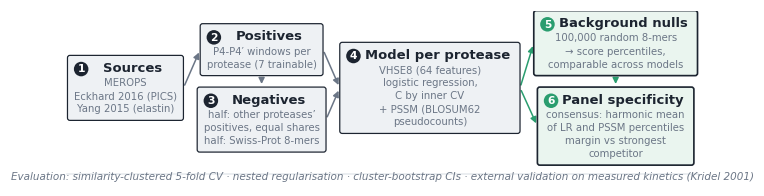
\includegraphics[width=\textwidth]{wiki_F01.png}
\caption{The pipeline from source data to a panel selectivity score: confirmed cleavage windows and constructed negatives train the logistic regression and PSSM for each protease, whose percentile scores combine into the consensus and specificity margin for a candidate peptide.}
\label{fig:pipeline}
\end{figure}

%=======================================================================
\section{Data}
\label{sec:data}
\subsection{MEROPS}

The MEROPS database contains data on the eight residues around the scissile bond (4 on each side) for each recorded cleavage of a given substrate. An example of the format of this data can be found at \url{https://www.ebi.ac.uk/merops/cgi-bin/substrates?id=M10.004}, for MMP-9.

We make the assumption here that the confirmed windows are correct positives. Treating MEROPS data as ground truth is valid as MEROPS is the standard curated database of protease cleavage sites, with each row being easily traced back to a published experiment.

From MEROPS, we use 2,318 windows for MMP-2, 96 for MMP-8, 341 for MMP-9, 129 for MMP-14, 327 for NE, 31 for LasB and 5,000 for the digestive serine proteases. There are 18,251 available windows for the digestive serine proteases, but we capped the set we use to 5,000 randomly chosen windows to avoid one group dominating the panel. Windows were also deduplicated.

One limitation of this method is that MEROPS combines physiological and synthetic substrates, and we didn't filter by evidence type in this iteration. Future work could inspect how the model's accuracy varies when considering purely physiological substrates.

\subsection{Eckhard 2016 (MMPs)}

Eckhard et al.~\cit{4} identified around 4,300 cleavage sites for 9 MMPs using proteomic peptide libraries. We used the data for MMP-2, MMP-8, MMP-9 and MMP-14. Each row from Eckhard gives the residue before the cut (P1) and the peptide after it, but not the full 8-letter window like MEROPS offers. To rebuild the window, we looked up the source protein in UniProt, found where the peptide sits and read the four residues on each side of the bond. 

The extra work for data reconciliation is well justified for the data on MMPs, particularly for the ones which have fewer documented cleavage sites in MEROPS. From Eckhard, we got 501 windows for MMP-2, 602 for MMP-8, 442 for MMP-9 and 588 for MMP-14.

\subsection{Yang 2015 (LasB)}

Yang et al.~\cit{5} is a study of how pseudolysin (LasB) degrades elastin. It lists 75 peptides, all of which have their start and end position in bovine tropoelastin, with residues just outside each end. We re-extracted the table from their PDF. To verify the correctness of our transcription, we checked that each peptide sits at its stated position in bovine tropoelastin from UniProt and that both flanking residues match, and all 75 did. As each peptide has two cut ends, we read the 8-letter window from the sequence around both, giving us 97 unique windows, which together with 31 windows from MEROPS make up the 128 LasB windows. The number of windows from each source for every protease is summarised in Table~\ref{tab:sources}.

\subsection{Negatives}

To build a strong classifier, we need examples of substrates that are not cleaved. No database records confirmed non-cleavage. We therefore construct our negatives, taking 3 negatives for every positive per target. For half of these negatives, we take other proteases' real windows, an equal share, excluding any windows that are the target's known positives. The other half of the negatives are random windows, built by picking each of the eight residues independently, using the natural amino acid frequencies in Swiss-Prot.

The major limitation of this method is the underlying assumption that, if a protease cleaves a given window and it is not a known window that our target protease cleaves, then our target protease doesn't cleave it. This is particularly likely among the MMP family, and treating such windows as negative penalises the model for something that may be true. We chose 3 to 1 and the half/half split, but future work could run ablation tests to see how the ratios affect the model's performance.

\begin{table}[H]
\centering
\small\renewcommand{\arraystretch}{1.2}
\begin{tabular}{@{}lrrrr@{}}
\toprule
Protease & MEROPS & Eckhard 2016 & Yang 2015 & Total \\
\midrule
MMP-2 & 2,318 & 501 & 0 & 2,819 \\
MMP-8 & 96 & 602 & 0 & 698 \\
MMP-9 & 341 & 442 & 0 & 783 \\
MMP-14 & 129 & 588 & 0 & 717 \\
Neutrophil elastase & 327 & 0 & 0 & 327 \\
LasB & 31 & 0 & 97 & 128 \\
Digestive serine proteases & 5,000 & 0 & 0 & 5,000 \\
\midrule
Total & 8,242 & 2,133 & 97 & 10,472 \\
\bottomrule
\end{tabular}
\caption{Confirmed cleavage windows per protease by source, after removing duplicate windows. A window reported by more than one source is counted once. The digestive serine protease set is capped at 5,000 of 18,251 available windows.}
\label{tab:sources}
\end{table}

%=======================================================================
\section{Models and Features}
\label{sec:features}

\subsection{Models}

As a brief overview, each of the seven proteases has two independent scoring models trained. One of these is a logistic regression on its physicochemical properties, and the other is a PSSM built from the observed amino-acid frequencies at each position.

Both of these are additive over the 8 positions, with the total score being a sum of one contribution per position. This matches how a protease recognises a substrate one binding pocket at a time.

These two scores are later combined into one comparable number per protease.

\subsection{Features}

We use the VHSE descriptors from Mei et al. 2005~\cit{6}, where each amino acid is converted into an 8-dimensional embedding. Mei took 18 hydrophobic, 17 steric and 15 electronic properties, and compressed them into 8 principal components via PCA, used to compress the data's dimensionality while capturing the maximal variance possible in fewer dimensions. The first 2 principal components (VHSE1-2) are hydrophobic, the next 2 (VHSE3-4) steric and the final 4 (VHSE5-8) electronic. This means that an 8-residue window becomes a 64-dimensional vector:
\begin{equation}
x(w) = [\varphi(w_1);\,\varphi(w_2);\,\dots;\,\varphi(w_8)] \in \mathbb{R}^{64},
\label{eq:x}
\end{equation}
where $\varphi(a)\in\R^8$ is the VHSE vector for residue $a$ and $w=(w_1,\dots,w_8)$ is the window.

Each of these 64 features is standardised, using the mean and standard deviation computed from the training data only, so that no property dominates the model due to its numeric scale.

\subsection{Model 1: Logistic Regression}

The first model used is logistic regression, one of the most explainable and simple machine learning models. We opted for logistic regression over a deep-learning approach as it is more interpretable and needs fewer examples to fit reliably, which is important as our smallest protease sets only have a few hundred positives.

It computes one weight per feature and an intercept, scored as a weighted sum passed through the logistic function ($\frac{1}{1+e^{-x}}$). Since there are three negatives for every positive, we weight positives with weight 2 and negatives with weight 2/3 during training, to avoid the model being influenced by the volume of negatives.

We use an L2 penalty on the weights, with the strength C chosen separately for each protease, using an inner cross-validation. For six of the seven proteases, the chosen strength lands at 0.01 or 0.1. The model is fit by minimising
\begin{equation}
\mathcal{L}(\bm\beta,b)=\tfrac12\|\bm\beta\|^2+C\sum_{i=1}^{n}\omega_{y_i}\log\bigl(1+e^{-\tilde y_i(\bm\beta^{\top}\bm z_i+b)}\bigr),\qquad \tilde y_i=2y_i-1,
\label{eq:lr}
\end{equation}
where $\bm z_i$ is the standardised feature vector of window $i$, $y_i\in\{0,1\}$ its label, and $\omega_{y_i}$ its class weight (2 for a positive, 2/3 for a negative). The first term is the L2 penalty (the sum of the squares of all 64 weights) and the second is the class-weighted log-loss; $C$ trades one off against the other. This loss is strictly convex, so the solver always finds the single global minimum.

As the score is linear in the 64 features, and the features are organised 8-per-position, the total logit splits exactly into one number per position, allowing us to say which positions of a peptide are driving its prediction:
\begin{equation}
\mathrm{logit}(w)=b+\sum_{i=1}^{8}\kappa_i(w),\qquad \kappa_i(w)=\sum_{d=1}^{8}\beta_{id}\,z_{id}(w),
\label{eq:decomp}
\end{equation}
where $\kappa_i(w)$ is position $i$'s contribution to the score, itself a weighted sum over that position's 8 standardised VHSE numbers $z_{id}(w)$.

\subsection{Model 2: PSSM}

A Position-Specific Scoring Matrix, or PSSM, is a table with position on one axis and the 20 amino acids on the other. In our case, we are considering 8 positions, so our table is 8 positions by 20 amino acids, where each cell tells us how much more or less likely a given amino acid is at a given position in a real cleavage site, compared with an ordinary protein. To score a window, we lookup the number for each of the 8 positions and add them, using the same additive structure as we did in the logistic regression.

For a position $i$ and amino acid $a$, we count how often $a$ appears in position $i$ among the known $n$ positives:
\begin{equation}
f_i(a) = \frac{n_i(a)}{n},
\label{eq:freq}
\end{equation}
where $n_i(a)$ is the number of positives with amino acid $a$ at position $i$. The limitation of this approach is that, when we consider a protease with only a few positives, like LasB with 128, many amino acids never appear at a given position by chance, giving $f_i(a)=0$. Plugging a 0 into a log-odds score later gives you $\log(0)$, which blows up. Even if it isn't zero, we accept there may be increasing noise as the number of positives we have decreases.

To try and fix this issue, we use BLOSUM62~\cit{7}, a standard table of how chemically/evolutionarily similar each pair of amino acids is. We take the observed frequencies and spread them through the similarity matrix by multiplying our frequency vector by the similarity matrix, giving us a weighted sum of the matrix's rows:
\begin{equation}
q_i = f_i W,
\label{eq:spread}
\end{equation}
where $W$ is BLOSUM62 with its negative entries removed and each row rescaled to sum to 1, so row $a$ of $W$ is a distribution over which amino acids are chemically similar to $a$. This means that, if an amino acid wasn't observed at a given position but a chemically similar one was, we have a nonzero estimate, rather than assuming it's impossible. We also have the background frequency $g$, which is how common each amino acid is in ordinary proteins, from Swiss-Prot.

We combine this into a weighted mix of the BLOSUM62-smoothed estimate and some of the plain background, as an extra safety net, with a weight of 0.05:
\begin{equation}
Q_i = (1-\epsilon)\,q_i + \epsilon\, g, \qquad \epsilon = 0.05.
\label{eq:mix}
\end{equation}

We then take a weighted average of the observed count's contribution and the smoothed prior's contribution for each position/amino acid combination, counting the prior as 5 extra observations:
\begin{equation}
p_i(a) = \frac{n\,f_i(a) + \beta\, Q_i(a)}{n+\beta}, \qquad \beta = 5.
\label{eq:pia}
\end{equation}

This means that when $n$ is large, our value tends towards the observed contribution, and tends towards the smoothed prior's contribution when $n$ is small.

For the score itself, we take the sum of the logs (base 2) of the ratio of $p_i(a)$ and how likely it is in an ordinary protein ($g$):
\begin{equation}
S(w) = \sum_{i=1}^{8} \log_2 \frac{p_i(w_i)}{g(w_i)}.
\label{eq:pssm_score}
\end{equation}
A positive contribution means that a given position favours cleavage more than chance would predict, and negative means it disfavours it.

Limitations of this method include $\beta$ and $\epsilon$ being fixed at 5 and 0.05, not being tuned by cross-validation like $C$ is for the logistic regression. Future work could consider ablation testing on these values.

\subsection{Making Scores Comparable}

We now have two types of models clearly defined, logistic regression and the PSSM, both of which give raw scores on different scales for different proteases, as each was trained on different data. Specifically, the mean logistic-regression score on random background windows ranges from 0.11 for digestive serine proteases to 0.35 for MMP-14 across the 7 models. So, comparing raw scores directly or taking a ratio isn't meaningful.

For a protease $k$, we let $F_k$ be the distribution of its score over 100,000 random background windows drawn from the Swiss-Prot natural amino acid frequencies, linearly interpolated through a 1,001-point quantile grid. The percentile of a window's score is just where it falls in that distribution, i.e. what fraction of random windows score lower than it:
\begin{equation}
u_k^{\mathrm{LR}}(w) = F_k^{\mathrm{LR}}\bigl(s_k^{\mathrm{LR}}(w)\bigr), \qquad u_k^{\mathrm{PSSM}}(w) = F_k^{\mathrm{PSSM}}\bigl(s_k^{\mathrm{PSSM}}(w)\bigr),
\label{eq:pct}
\end{equation}
giving two separate percentiles for each protease, one from logistic regression and one from the PSSM.

Because each percentile is, by construction, uniform on $[0,1]$ under the null, percentiles from different proteases and scorers are now directly comparable, unlike the raw scores.

A limitation of this method is that we use 100,000 background windows, while using 1,000,000 or 10,000,000 would converge closer to the true distribution, especially in the tails, which matter most for extreme percentiles. We chose 100,000 to keep the time taken to fit the distribution reasonable. 

As mentioned before, we have two percentiles for each protease, which we need to combine. A simple approach would be to take the arithmetic mean of the two numbers, but we want consensus, so if a value is low on one score and quite high on the other, the arithmetic mean doesn't capture that idea. A much more unforgiving option is the harmonic mean, defined as:
\begin{equation}
u_k(w) = \frac{2\, u_k^{\mathrm{LR}}(w)\, u_k^{\mathrm{PSSM}}(w)}{u_k^{\mathrm{LR}}(w) + u_k^{\mathrm{PSSM}}(w)}.
\label{eq:cons}
\end{equation}

The harmonic mean is more sensitive to the smaller of the two numbers, only high when both numbers are high, making this a much better metric to use. This is a more conservative choice but hopefully increases the reliability of our output, increasing the specificity of our modelling, the goal we laid out from the beginning. It is worth noting that this was just a reasoned decision, not tuned for selectivity.

The final number we output is the specificity margin, the target's consensus percentile minus whatever competitor scores it highest, ranging from $-1$ to $+1$:
\begin{equation}
M_t(w) = u_t(w) - \max_{j \neq t} u_j(w).
\label{eq:margin}
\end{equation}

Near $+1$, the peptide is in the extreme tail for the target and looks normal to every competitor, making it incredibly selective.

Near $0$, at least one other competitor scores it around as strongly as the target, making it not selective.

\begin{figure}[H]
\centering
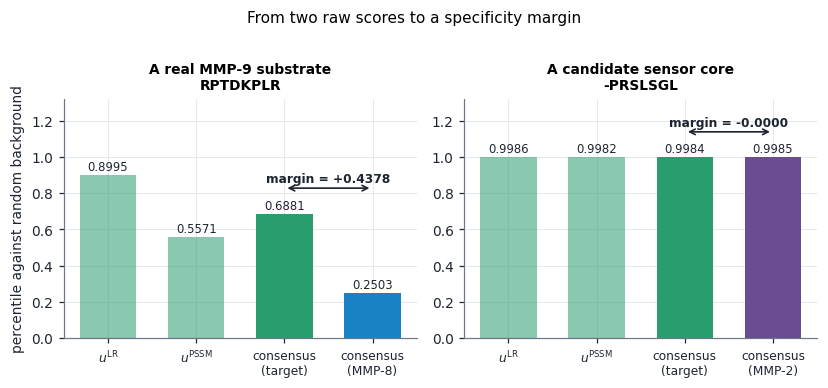
\includegraphics[width=\textwidth]{wiki_figW1.png}
\caption{Two real windows, worked through Equations~\ref{eq:pct}--\ref{eq:margin}. \textbf{Left:} a confirmed MMP-9 substrate, RPTDKPLR: its two percentiles combine into a consensus of 0.69 for the target, well above its strongest competitor's 0.25, giving a large positive margin. \textbf{Right:} candidate sensor core -PRSLSGL: the target and its strongest competitor (MMP-2) score almost identically, so the margin is close to zero, i.e. not selective.}
\label{fig:margin_example}
\end{figure}

A limitation of this is that the margin is defined relative to competitors, so adding or removing a competitor changes the margin and requires recomputation.

A complication is that many of our real sensor candidates are shorter than 8 residues, so at least one position doesn't have an amino acid to plug in. 

For the logistic regression model, an unknown position is filled with `the average residue', which, given that our features are standardised, is exactly 0. It therefore contributes nothing to the total logit, treated as neutral.

For the PSSM, we take the weighted average over all 20 amino acids, weighted by how common each is naturally (the background frequency $g$), i.e. what you'd expect on average if you had to guess the residue randomly given natural frequencies:
\begin{equation}
\sum_{a} g(a) \log_2 \frac{p_i(a)}{g(a)}.
\label{eq:gap_pssm}
\end{equation}

Shorter peptides can crop up if a designed peptide's cleavage bond doesn't sit in the middle of the 8-residue frame, or if a real substrate sits near the very end of its parent protein. Without this fix for shorter peptides, we wouldn't be able to reliably model these situations.

\subsection{Assumptions and Limitations}

Here is a summary of assumptions and limitations of the models and scoring pipeline described above:

\begin{assump}
\begin{itemize}[leftmargin=*]
\item \textbf{Positions act independently (additivity).} The scorers assume that each position acts independently, that there is no interaction between positions. A model that can capture interactions (gradient-boosted trees) beats the additive model by no more than 0.007 AUROC on any protease.
\item \textbf{The VHSE descriptors are a compression, not the full picture.} The dimensionality reduction by PCA on the original VHSE descriptors captures between 64\% and 79\% of the position-specific signal that a full, uncompressed encoding could capture.
\item \textbf{$C$ is tuned, but only over a fixed grid.} We use a log-spaced grid instead of a fully continuous search for tuning C.
\item \textbf{$\beta$ and $\epsilon$ are fixed, not tuned.} Unlike $C$, we don't tune these variables with cross-validation.
\item \textbf{Random Swiss-Prot windows stand in for ``non-substrates''.} Some random windows may be real substrates, which would quietly lower percentiles.
\item \textbf{100,000 background windows is a time/accuracy trade-off.} Using a higher number of background windows would improve the accuracy of our fitted distribution, at the cost of much more computation time.
\item \textbf{The harmonic-mean consensus was reasoned, not tuned or validated.} This wasn't tuned or validated against any selectivity ground truth.
\item \textbf{The margin is defined relative to a chosen panel.} These margins are not absolute, by construction. Any changes to the panel require recomputation of all margins, making it difficult to generalise our results to other panels.
\end{itemize}
\end{assump}


%=======================================================================
\section{Evaluation}
\label{sec:evaluation}

\subsection{Cross-Validation Design}

$K$-fold cross validation is distinct from a typical train-test split as, instead of having a pre-defined train and test set, we split our data into $K$ folds, train on $K-1$ of them, and test on the 1 left out. We repeat this $K$ times with fresh models, each testing on a different fold, so each window gets tested exactly once. We pool those test predictions together to get one full evaluation of every window in our dataset.

The limitation of this is that it assumes that every window is genuinely independent of other windows. Here that is false - there are many near-duplicate windows, meaning that it may see incredibly similar peptides in the train set and score a similar peptide well without having to learn anything general. This doesn't measure generalisation well, and ends up being a form of data leakage.

We use the Hamming distance to describe clusters, defined as the number of positions where two strings of equal length differ. For two windows $w=(w_1,\dots,w_8)$ and $w'=(w_1',\dots,w_8')$,
\begin{equation}
d_H(w,w') = \bigl|\{\, i : w_i \neq w_i' \,\}\bigr|,
\label{eq:hamming}
\end{equation}
simply the count of positions at which the two windows disagree. We treat any pair with $d_H(w,w') \leq 2$ as close enough to leak, so we define a cluster as a connected component of this relationship: the set of all peptides that can be reached by traversing edges connecting peptides with $d_H \leq 2$ together, meaning that we account for leakage travelling through the chain.

After this, we construct a stratified group 5-fold, splitting entire clusters into folds, so they stay together, never split across train and test, removing any leakage. We aim to keep the ratio of positives to negatives roughly equal across all 5 folds.

The next item is the nested inner cross-validation. We mentioned how the model needs to tune its regularisation strength $C$, so we nest a smaller cross-validation within the training data, splitting it into three inner folds and choosing
\begin{equation}
C^\star = \operatorname*{arg\,max}_{C \in \{10^{-3},10^{-2},10^{-1},1,10,10^{2}\}} \overline{\mathrm{AUROC}}_{\mathrm{inner}}(C),
\label{eq:cstar}
\end{equation}
where $\overline{\mathrm{AUROC}}_{\mathrm{inner}}(C)$ is the mean AUROC across the 3 inner folds when the model is trained with regularisation strength $C$, then refitting the model on the full outer training set with that chosen $C^\star$.

We also rebuild the null percentile distribution and PSSM for each outer fold, using only that fold's training positives, to avoid any leakage into the background distribution.

\subsection{AUROC}

We use AUROC as our primary metric throughout this pipeline. It is the probability that a randomly chosen positive scores higher than a randomly chosen negative, defined formally, for $n_+$ positives and $n_-$ negatives with scores $s(x_i^+)$ and $s(x_j^-)$, as:
\begin{equation}
\mathrm{AUROC} = \frac{1}{n_+ n_-} \sum_{i=1}^{n_+}\sum_{j=1}^{n_-}
\begin{cases}
1 & s(x_i^+) > s(x_j^-) \\
\tfrac12 & s(x_i^+) = s(x_j^-) \\
0 & s(x_i^+) < s(x_j^-)
\end{cases}
\label{eq:auroc}
\end{equation}
i.e. we look at every possible pairing of one positive with one negative, count how often the positive scores higher (a tie counting as half a win), and average over all $n_+n_-$ pairs.

We pick this metric as it is threshold-free, not requiring a cutoff above which you would call something cleaved. It is also invariant to monotone rescaling, as any order-preserving transformation wouldn't change the AUROC, as we only really care about the ranking here. It isn't affected by class ratio as well - plain accuracy would be skewed towards collapsing to a single class label, while AUROC doesn't have that failure mode.

We care about two things when it comes to out-of-fold predictions. The first is Detection - are held-out confirmed sites ranked above random background windows? The second is Discrimination - are these confirmed sites ranked above another protease's confirmed sites? Discrimination is the harder of the two, but is the one that really matters for a multiplexed sensor.

We assume negatives, instead of confirming them, as detailed in the Data section. Suppose a fraction $\pi$ of our labelled negatives are actually false negatives (genuinely cleaved by the target and mislabelled). What would this do to the AUROC?

The measured AUROC compares a real positive $X$ against a random draw from the labelled-negative pool. With probability $1-\pi$ that draw is a true negative $Y_{\mathrm{true}}$, and with probability $\pi$ it is a hidden positive $Y_{\mathrm{hidden}}$ (another genuine positive, just mislabelled). This means that measured AUROC is:
\begin{equation}
\mathrm{AUROC}_{\mathrm{measured}} = (1-\pi)\,\Prob\bigl(s(X) > s(Y_{\mathrm{true}})\bigr) + \pi\,\Prob\bigl(s(X) > s(Y_{\mathrm{hidden}})\bigr).
\label{eq:auroc_noisy}
\end{equation}
By definition, the first term is exactly the true AUROC. The second term compares two windows both from the same distribution, and by symmetry, for two independent draws from the same distribution, $\Prob(s(X) > s(Y)) = \Prob(s(Y) > s(X))$, and since these sum to 1, each equals $\tfrac12$. So measured AUROC is
\begin{equation}
\mathrm{AUROC}_{\mathrm{measured}} = (1-\pi)\,\mathrm{AUROC}_{\mathrm{true}} + \frac{\pi}{2}.
\label{eq:auroc_final}
\end{equation}
And since AUROC can be at most 1, as it is a probability,
\begin{equation}
\mathrm{AUROC}_{\mathrm{measured}} \leq (1-\pi)(1) + \frac{\pi}{2} = 1 - \frac{\pi}{2}.
\label{eq:auroc_bound}
\end{equation}
Thus, even a perfect model cannot score above $1-\pi/2$ on this measurement, meaning that some of the imperfection is likely due to the effect of assuming negatives.

We compute confidence intervals from a cluster bootstrap, resampling clusters with replacement, recomputing AUROC and taking the resulting spread as the interval. 

\begin{figure}[H]
\centering
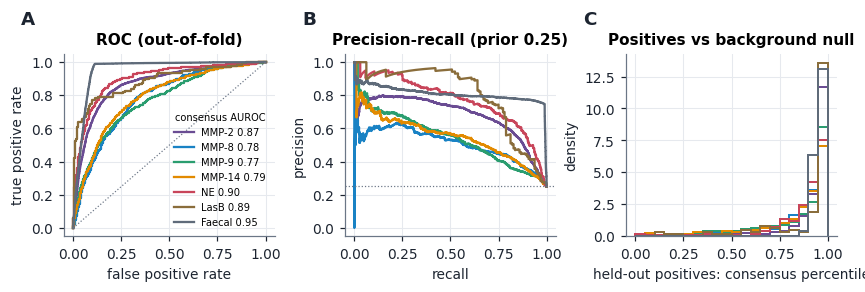
\includegraphics[width=\textwidth]{wiki_F09.png}
\caption{Out-of-fold performance of the consensus score, for all seven proteases. \textbf{A:} ROC curves (true positive rate against false positive rate), with each protease's detection AUROC in the legend. \textbf{B:} precision-recall curves, against a 0.25 prior (dotted line). \textbf{C:} the distribution of held-out positives' consensus percentiles against the background null - a model with no detection ability would look uniform on $[0,1]$, matching the null it is compared against.}
\label{fig:roc_pr}
\end{figure}

\subsection{Controls}

We ran three checks, each answering a question about whether a given result is real.

The first is a label-shuffle control, randomly permuting labels before training. AUROC collapses to 0.49 to 0.53 across all 7 proteases, essentially chance, proving that there is real learning happening.

The second is a composition only control. We check how well a model given only the peptide's overall amino acid composition, without any positional information. The results here are mixed. For most proteases, there is a huge gap, for example 0.664 vs 0.874 for MMP-2, but for LasB, composition-only at 0.886 matches or slightly exceeds the full logistic regression (0.877) and PSSM (0.881). This likely ties back to 76\% of LasB's positives come from elastin, with elastin's composition specific enough on its own that position-specific information isn't adding much. There are also very few LasB positives compared to other proteases.

\begin{figure}[H]
\centering
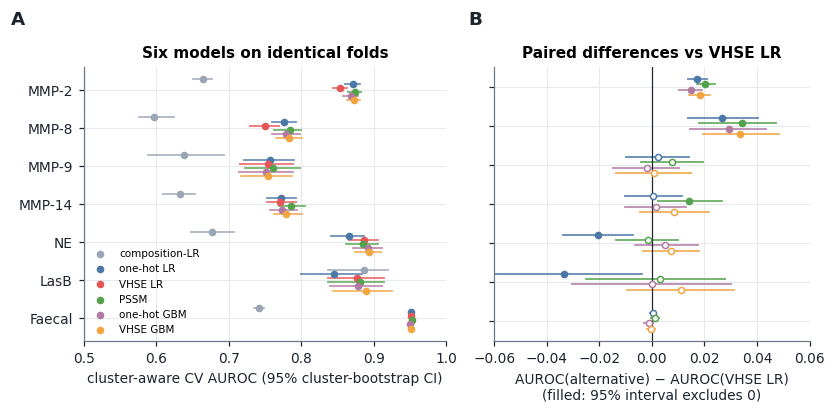
\includegraphics[width=\textwidth]{wiki_F05.png}
\caption{\textbf{A:} cluster-aware CV AUROC (95\% cluster-bootstrap interval) for six models on identical folds per protease: composition-only, one-hot LR, VHSE LR, PSSM, one-hot GBM and VHSE GBM. \textbf{B:} paired differences against VHSE LR for the four alternative models, per protease; a filled marker means the 95\% interval excludes 0, i.e. a statistically resolvable difference.}
\label{fig:model_comparison}
\end{figure}

The final check is a fold-construction control, comparing plain random folds against our cluster-aware folds. For most proteases the difference is tiny, with MMP-9 at 0.755 random and 0.756 clustered, but LasB has the largest gap, with 0.886 random and 0.879 clustered, a measurable drop once leakage is removed - direct evidence that the clustering matters.

%=======================================================================
\section{Results}
\label{sec:results}

\subsection{Detection Performance}

\begin{table}[H]
\centering
\footnotesize\renewcommand{\arraystretch}{1.25}
\begin{tabular}{@{}lrccc@{}}
\toprule
Protease & Positives (clusters) & LR AUROC & PSSM AUROC & Consensus AUROC \\
\midrule
MMP-2 & 2,819 (2,608) & 0.854\,[0.844, 0.863] & \textbf{0.874}\,[0.863, 0.883] & 0.869\,[0.859, 0.878] \\
MMP-8 & 698 (677) & 0.755\,[0.733, 0.774] & \textbf{0.784}\,[0.762, 0.800] & 0.783\,[0.763, 0.800] \\
MMP-9 & 783 (687) & 0.760\,[0.723, 0.791] & 0.761\,[0.723, 0.798] & \textbf{0.772}\,[0.737, 0.803] \\
MMP-14 & 717 (705) & 0.772\,[0.753, 0.790] & 0.785\,[0.766, 0.806] & \textbf{0.791}\,[0.771, 0.810] \\
Neutrophil elastase & 327 (324) & 0.895\,[0.875, 0.913] & 0.885\,[0.861, 0.906] & \textbf{0.901}\,[0.880, 0.919] \\
LasB & 128 (106) & 0.877\,[0.835, 0.917] & 0.881\,[0.837, 0.916] & \textbf{0.887}\,[0.844, 0.923] \\
Digestive serine proteases & 5,000 (4,715) & 0.951\,[0.948, 0.954] & \textbf{0.953}\,[0.950, 0.956] & \textbf{0.953}\,[0.950, 0.956] \\
\bottomrule
\end{tabular}
\caption{Out-of-fold detection AUROC per protease (95\% cluster-bootstrap intervals), against the standard held-out negative pool. Positives (clusters) shows the number of confirmed positives and, in brackets, the number of Hamming-distance clusters they form. Bold marks the best of the three scores for each protease.}
\label{tab:detection}
\end{table}

The consensus AUROC range goes from 0.77 for MMP-9 to 0.95 for the digestive serine proteases. The consensus rarely underperforms both individual scorers, modest empirical validation of the choice to use the harmonic mean. This addresses the detection question, not the discrimination one, detecting against the standard held-out negative pool.

\subsection{Selectivity Between Proteases}

\begin{table}[H]
\centering
\footnotesize\renewcommand{\arraystretch}{1.25}
\begin{tabular}{@{}lccccccc@{}}
\toprule
Target $\downarrow$ / Competitor $\rightarrow$ & MMP-2 & MMP-8 & MMP-9 & MMP-14 & NE & LasB & Digestive serine \\
\midrule
MMP-2 & -- & 0.72 & 0.68 & 0.69 & 0.93 & 0.79 & 0.89 \\
MMP-8 & 0.57 & -- & 0.58 & 0.64 & 0.91 & 0.82 & 0.63 \\
MMP-9 & 0.59 & 0.65 & -- & 0.70 & 0.90 & 0.63 & 0.63 \\
MMP-14 & 0.53 & 0.62 & 0.70 & -- & 0.89 & 0.80 & 0.84 \\
Neutrophil elastase & 0.93 & 0.93 & 0.93 & 0.94 & -- & 0.92 & 0.96 \\
LasB & 0.84 & 0.90 & 0.81 & 0.84 & 0.87 & -- & 0.91 \\
Digestive serine proteases & 0.96 & 0.90 & 0.91 & 0.96 & 0.98 & 0.97 & -- \\
\bottomrule
\end{tabular}
\caption{Pairwise discrimination AUROC: each row's model separating its own confirmed positives from the column protease's confirmed positives.}
\label{tab:selectivity}
\end{table}

Among the four MMPs, pairwise discrimination is weak, barely better than chance in some instances. Against neutrophil elastase, every MMP does well. MMP-9 is a mixed case, strong against NE, weak against the other MMPs as expected, but also 0.63 against LasB and the digestive serine proteases, a limitation of the MMP-9 model, potentially related to having fewer positives than other MMPs.

\begin{figure}[H]
\centering
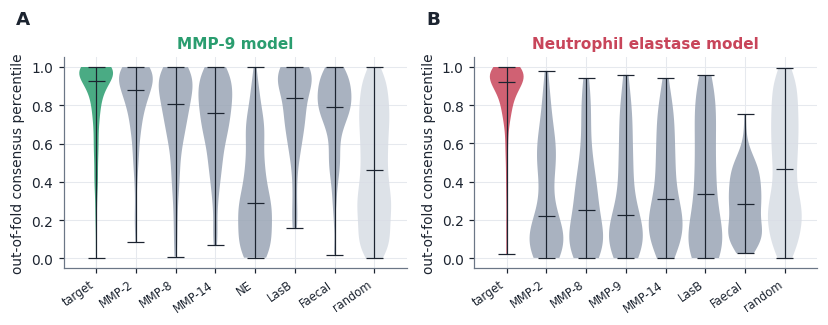
\includegraphics[width=\textwidth]{wiki_F16.png}
\caption{Out-of-fold consensus percentiles of held-out positives (``target'') compared with each competitor's confirmed windows and with random background windows. \textbf{A:} the MMP-9 model - the target distribution overlaps heavily with MMP-2 and MMP-8. \textbf{B:} the NE model, for comparison - the target distribution is well separated from every competitor.}
\label{fig:score_dist}
\end{figure}

Exact window overlap between proteases is small, with a maximum Jaccard index of 0.145, but the learned preferences overlap strongly, with MMP-2, MMP-8 and MMP-14 PSSM log-odds vectors correlating at $r$ between 0.73 and 0.82 with each other, MMP-9 correlating at $r$ between 0.56 and 0.63 with each of them. NE is essentially uncorrelated with the MMPs and correlates with the digestive serine proteases at only 0.46, both being serine proteases but still fairly distinct.

\begin{figure}[H]
\centering
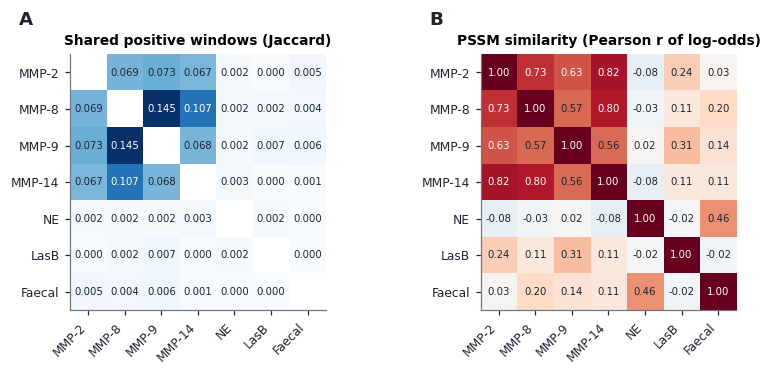
\includegraphics[width=\textwidth]{wiki_F04.png}
\caption{\textbf{A:} Jaccard index of exact shared positive windows between each pair of proteases - low throughout. \textbf{B:} Pearson correlation of the $8\times20$ PSSM log-odds vectors between each pair - high among the four MMPs, low between NE and the MMPs, showing that the overlap is in learned preference, not in shared training windows.}
\label{fig:similarity}
\end{figure}

The key takeaway from this is that the models aren't failing to learn. MMPs do genuinely share a recognition motif, so their PSSMs converge on similar preference, which explains why pairwise discrimination is a fundamentally hard problem as opposed to a modelling flaw.

\subsection{Independent Validation}

Kridel et al. 2001~\cit{1} measured actual MMP-9 cleavage rates for 11 synthetic peptides, and found no detectable activity on a 12th. Any training window sharing 7+ of 8 positions with one of the four validation peptides was stripped from training, the MMP-9 model retrained before scoring, the same Hamming-distance logic as the cross-validation design. As the cleavage rate is continuous, we use the Spearman rank correlation between model score and $\log_{10}(\kcat/\Km)$. Spearman correlation is simply the Pearson correlation computed on the ranks of the two variables rather than their raw values, so it only cares about whether a higher score corresponds to a higher measured rate, not about the exact relationship between them, which is appropriate here since we have no reason to expect a linear relationship between the two. For $n$ paired observations, with $d_i$ the difference between the rank of the model score and the rank of the measured rate for peptide $i$,
\begin{equation}
\rho = 1 - \frac{6\sum_{i=1}^{n} d_i^2}{n(n^2-1)}.
\label{eq:spearman}
\end{equation}

\begin{table}[H]
\centering
\footnotesize\renewcommand{\arraystretch}{1.25}
\begin{tabular}{@{}llccc@{}}
\toprule
Score & Set & Spearman $\rho$ & 95\% CI & Permutation $p$ \\
\midrule
Logistic regression & $n=11$ measured & 0.58 & [$-0.23$, 0.93] & 0.068 \\
Logistic regression & $n=12$ (C11 ranked lowest) & 0.68 & [0.02, 0.96] & 0.017 \\
PSSM & $n=11$ measured & 0.70 & [$-0.00$, 0.96] & 0.020 \\
PSSM & $n=12$ (C11 ranked lowest) & 0.75 & [0.18, 0.93] & 0.006 \\
\bottomrule
\end{tabular}
\caption{Spearman rank correlation between model score and measured $\log_{10}(\kcat/\Km)$ on the Kridel et al.\ peptides, with permutation $p$-values and bootstrap confidence intervals over peptides.}
\label{tab:kridel}
\end{table}

\begin{figure}[H]
\centering
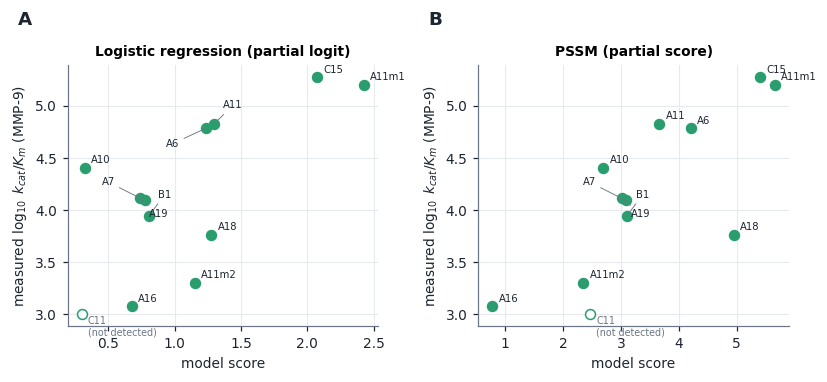
\includegraphics[width=\textwidth]{wiki_F15.png}
\caption{Model score against measured MMP-9 $\log_{10}(\kcat/\Km)$, for the logistic regression (left) and the PSSM (right). Open marker: C11, no activity detected, plotted at the floor of the axis.}
\label{fig:kridel_val}
\end{figure}

As n is small, Kridel's peptides were themselves selected for high activity rather than randomly sampled, and the logistic regression result at n=11 has a confidence interval including 0. This is evidence of a positive association, but importantly not a proof of accurate rate prediction.

Logistic Regression's top 3 scored peptides are genuinely the 3 most active ones measured, a pleasing agreement to see at the top. Its biggest miss was the 5th most active one, which it scored as second-lowest.

\subsection{Sensor Candidates}

\begin{table}[H]
\centering
\footnotesize\renewcommand{\arraystretch}{1.25}
\begin{tabular}{@{}llccccc@{}}
\toprule
Candidate & Core & Target & $u_{\text{MMP-2}}$ & $u_{\text{MMP-9}}$ & $u_{\text{NE}}$ & Margin \\
\midrule
Cand1\_MMP9 & PRSLSGLK & MMP-9 & 0.9985 & 0.9984 & 0.1529 & $-0.0001$ \\
Cand2\_MMP2 & PLGLAGQS & MMP-2 & 0.9984 & 0.9992 & 0.0012 & $-0.0008$ \\
Cand3\_MMP2b & PLGVALAA & MMP-2 & 0.9450 & 0.9817 & 0.0274 & $-0.0367$ \\
Cand4\_NE & AAPVSGIG & NE & 0.0658 & 0.4872 & 0.9979 & $+0.5107$ \\
\bottomrule
\end{tabular}
\caption{Consensus percentiles of the four sensor candidates against the 3-plex panel (MMP-2, MMP-9, NE), the panel actually used in the sensor design, narrower than the wound panel used earlier in Results. Margin is computed from Equation~\ref{eq:margin}: the target's percentile minus its strongest competitor's.}
\label{tab:candidates}
\end{table}

Every single MMP-targeted candidate has a margin at or below 0. Only the neutrophil elastase candidate, not competing against any shared recognition motif, achieves real separation.

%=======================================================================
\section*{References}

\begin{enumerate}[label={[\arabic*]},noitemsep,leftmargin=*]
\item Kridel SJ, Chen E, Kotra LP, Howard EW, Mobashery S, Smith JW (2001).
  Substrate hydrolysis by matrix metalloproteinase-9.
  \textit{J Biol Chem} 276(23):20572--20578.

\item Nagase H, Woessner JF Jr (1999). Matrix metalloproteinases.
  \textit{J Biol Chem} 274(31):21491--21494.

\item Trengove NJ, Stacey MC, MacAuley S, Bennett N, Gibson J, Burslem F,
  Murphy G, Schultz G (1999). Analysis of the acute and chronic wound
  environments: the role of proteases and their inhibitors.
  \textit{Wound Repair Regen} 7:442--452.

\item Eckhard U, Huesgen PF, Schilling O, Bellac CL, Butler GS, Cox JH, Dufour A,
  Goebeler V, Kappelhoff R, Keller UAD, Klein T, Lange PF, Marino G, Morrison CJ,
  Prudova A, Rodriguez D, Starr AE, Wang Y, Overall CM (2016). Active site
  specificity profiling of the matrix metalloproteinase family: proteomic
  identification of 4300 cleavage sites by nine MMPs explored with structural and
  synthetic peptide cleavage analyses. \textit{Matrix Biol} 49:37--60.

\item Yang J, Zhao HL, Ran LY, Li CY, Zhang XY, Su HN, Shi M, Zhou BC, Chen XL,
  Zhang YZ (2015). Mechanistic insights into elastin degradation by pseudolysin,
  the major virulence factor of the opportunistic pathogen \textit{Pseudomonas
  aeruginosa}. \textit{Sci Rep} 5:9936.

\item Mei H, Liao ZH, Zhou Y, Li SZ (2005). A new set of amino acid descriptors
  and its application in peptide QSARs. \textit{Biopolymers} 80(6):775--786.

\item Henikoff S, Henikoff JG (1992). Amino acid substitution matrices from
  protein blocks. \textit{Proc Natl Acad Sci USA} 89:10915--10919.
\end{enumerate}

\end{document}
